\documentclass[aspectratio=169,shadow=true]{beamer}
% \usepackage{beamerthemesplit} % Activate for custom appearance
\usepackage{amsmath}
\usepackage{siunitx}
\usepackage{listings}
\usepackage{pdfpages}
\usepackage[export]{adjustbox}
\usetheme{Boadilla}
\usepackage{ecuPresentation}



\title[ECU online labs]{Transition to online labs at ECU}
\author[Sprague and Wolf]{Mark W.\ Sprague and Steven F.\ Wolf}
\institute[ECU]{East Carolina University}
\date{\today}

\definecolor{light-gray}{gray}{0.95}
\newcommand{\code}[1]{\colorbox{light-gray}{\texttt{#1}}}

%\renewcommand*{\thefootnote}{\fnsymbol{footnote}}

\begin{document}

\begin{frame}
  \titlepage
\end{frame}

\begin{frame}
  {Transition to online labs at ECU}
  \tableofcontents
\end{frame}

\section{Labs before Coronavirus}
\begin{frame}{ECU's Lab transformation grant -- XLABs (Awarded 2017)}
  \noindent
  \begin{minipage}{0.35\textwidth}\scriptsize
    \begin{block}{Team Members}
      Physics:
      \begin{itemize}
        \item Co-PI: Steven Wolf
        \item Mark Sprague
      \end{itemize}
      Chemistry:
      \begin{itemize}
        \item Project Lead: Joi Walker
        \item Rosa Bell
        \item Kate Hosbein
        \item Annalisa Smith-Joyner
        \item Eric Eaton
      \end{itemize}
      Biology:
      \begin{itemize}
        \item Co-PI: Heather Vance-Chalcraft
        \item Co-PI: Kristine Callis-Duehl
        \item Taria Crenshaw
      \end{itemize}
    \end{block}
  \end{minipage}\hfill%
  \begin{minipage}[b]{0.6\textwidth}\scriptsize
    \begin{block}{Project page:}
      \centering \url{http://blog.ecu.edu/sites/xlabs/}
    \end{block}
    \begin{center}
      \begin{tabular}{ccc}
        
\includegraphics[width=0.25\textwidth]{./logos/NSF_4-Color_bitmap_Logo.png}
        &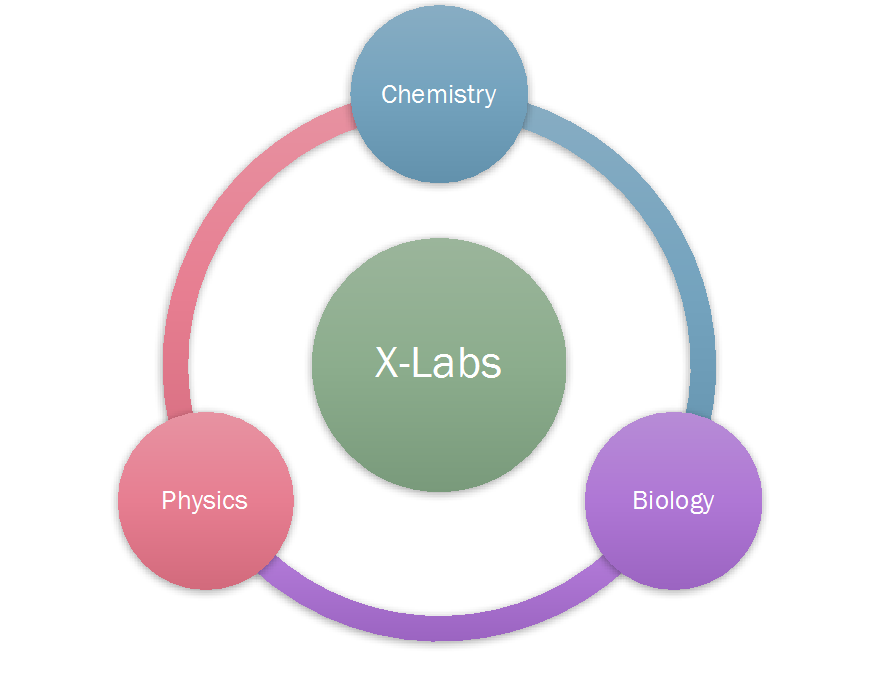
\includegraphics[width=0.3\textwidth,trim = 60 0 70 0, clip]{./logos/xlabsLogo.png}%
        &
\includegraphics[width=0.25\textwidth]{./logos/stemCoreLogoTall.pdf}\\
          Award \# 1725655
      \end{tabular}
    \end{center}
  \end{minipage}

  
  \begin{minipage}{0.2\textwidth}
  \end{minipage}\hspace{0.4in}%
  \begin{minipage}{0.5\textwidth}%
  \end{minipage}
\end{frame}

{\nologo
\begin{frame}
  \frametitle{Physics labs at ECU in BC days}
  \begin{center}
    \only<1>{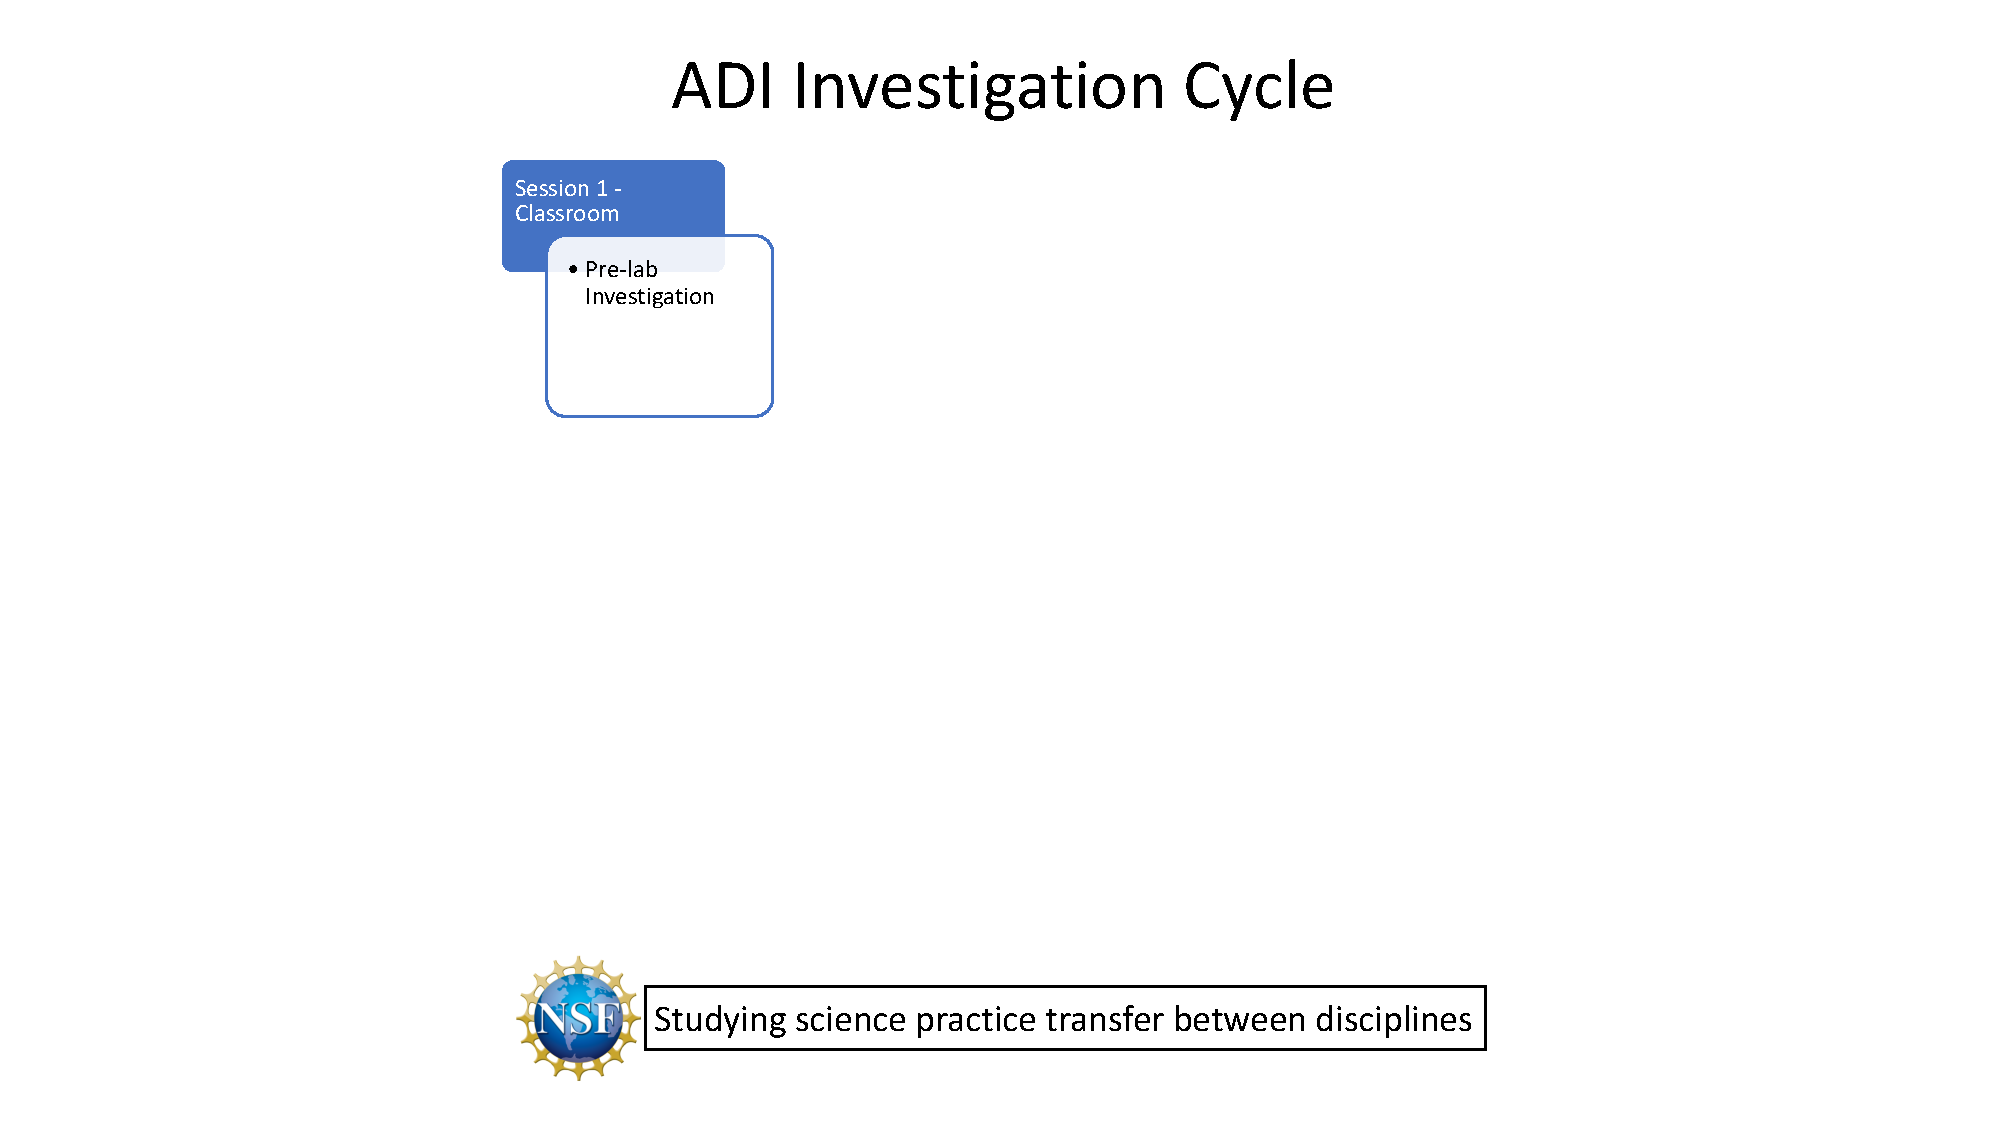
\includegraphics[page=1, height=3in, valign=m]{PICUP1.pdf}}
    \only<2>{\includegraphics[page=2, height=3in, valign=m]{PICUP1.pdf}}
    \only<3>{\includegraphics[page=3, height=3in, valign=m]{PICUP1.pdf}}
    \only<4>{\includegraphics[page=4, height=3in, valign=m]{PICUP1.pdf}}
  \end{center}
\end{frame}
}

\section{Spring 2020:  Adapt! (Don't change)}
\begin{frame}
  \frametitle{Spring 2020:  Adapt! (Don't change)}
  \begin{center}
    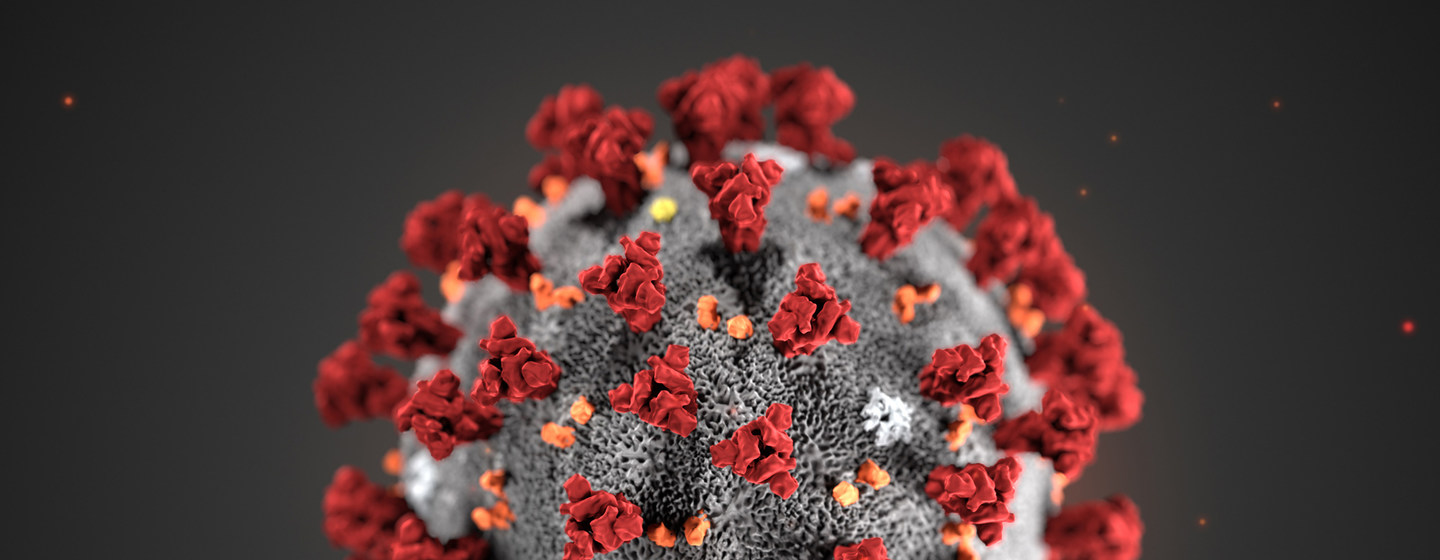
\includegraphics[width=2in]{coronavirus.jpg}
  \end{center}
  \begin{itemize}
    \item<1-> Preserve ADI format for last two investigations
    \item<1-> How can we change our delivery while maintaining our focus on science practices?
    \item<2-> What do we need to do together? (What requires active approval?)
    \begin{enumerate}
      \item Proposal approval
      \item Argumentation session
    \end{enumerate}
    \item<3-> What can we do apart? (What do we want students to solve on their own?)
    \begin{enumerate}
      \item Data collection (Both Prelab and Inquiry Investigation)
      \item Data analysis
      \item Peer review/lab report revision
    \end{enumerate}
  \end{itemize}
\end{frame}

\begin{frame}
  \frametitle{Delivering Data}
  \begin{center}
    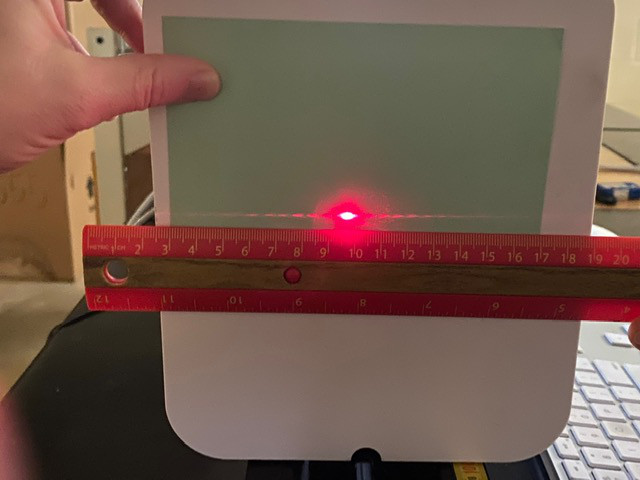
\includegraphics[width=2in]{Hair1_red_pattern.jpg}\\
    {\footnotesize Image of diffraction pattern for student measurement.}
  \end{center}
  \begin{itemize}
    \item Measurements online using photos and
    \href{https://ecu.instructuremedia.com/embed/7b72631f-ea1e-4c4d-a0bd-642c4a2d0356}{video}
    \item Simulations on \emph{Trinket}
  \end{itemize}
\end{frame}

\begin{frame}
  \frametitle{Challenges with online labs}
  \begin{block}{Technology-based}
    Used university-supported solutions or open-source software
    \begin{itemize}
      \item Microsoft Office (Excel)
      \item Tracker
      \item ImageJ
    \end{itemize}
    Required students to install on their own machines.
    \begin{itemize}
      \item ECU Center for Survey research identified access to computers as an issue for a
      significant fraction of our students. (Nearly 2000)
      \item Not all computers are created equal. (Chromebooks were a problem)
    \end{itemize}
  \end{block}
\end{frame}

\begin{frame}
  \frametitle{Challenges with online labs}
  \begin{block}{Curriculum-based}
    Argumentation sessions got quiet
    \begin{itemize}
      \item Participation in argumentation was more muted
      \item Fewer questions, less sharing ideas
    \end{itemize}
  \end{block}
\end{frame}

\section{Fall 2020 (and beyond?)}
{\nologo
\begin{frame}
  \frametitle{Fall 2020 plans (and beyond)?}
  \begin{block}{Goal:  We still wanted a hands on experience.}
    Adaptations for fully online labs:
    \begin{itemize}
      \item Lab manuals were made available online
      \item Students purchased kits for a reasonable price
      \item Activities/questions slightly changed
    \end{itemize}
    Post pandemic: We have DE students who struggle to take lab courses.
  \end{block}
  \begin{block}{Adaptations to challenges}
    \begin{itemize}
      \item Students are made aware of computing requirements/work-arounds
      \item Argumentation sessions became a participation grade
    \end{itemize}
  \end{block}
\end{frame}
}

\begin{frame}
  \frametitle{Fall 2020 plans (and beyond)}
  \begin{block}{New challenge:  8 week blocks}
    \begin{itemize}
      \item We dropped an investigation
      \item We added some pre-labs
    \end{itemize}
    This helped with grading.
  \end{block}
\end{frame}

{\nologo
  \begin{frame}
    \frametitle{Tools used in online lab delivery}
    \begin{center}
      \renewcommand{\arraystretch}{1.5}
      \begin{tabular}{cll}
        \hline\hline
        \textbf{Tool} & \textbf{Use} & \textbf{Rationale} \\
        \hline
        Canvas & \parbox[t]{2in}{\raggedright Material, Assignments, Quizzes, Discussions,
                 Online Peer Review }& University LMS\\
        WebEx & \parbox[t]{2in}{\raggedright Class introduction, argumentation, group interactions (???)} & University supported\\
        Trinket.io & \parbox[t]{2in}{\raggedright Simulations embedded in Canvas} &
                                                                                    Fine-grained
                                                                                    control\\
        ImageJ &Image processing software &Open-source \\
        Tracker &Video processing software &Open-source \\
        \hline\hline
      \end{tabular}
    \end{center}
  \end{frame}
}

\end{document}
